\begin{mainquestion}{circuit_001}{Circuit Solving}
Continuing the problem from the previous homework, steel yourself for some math!  You will use KCL, KVL and Ohm’s law to determine the voltage and current of each branch element.

\begin{center}
    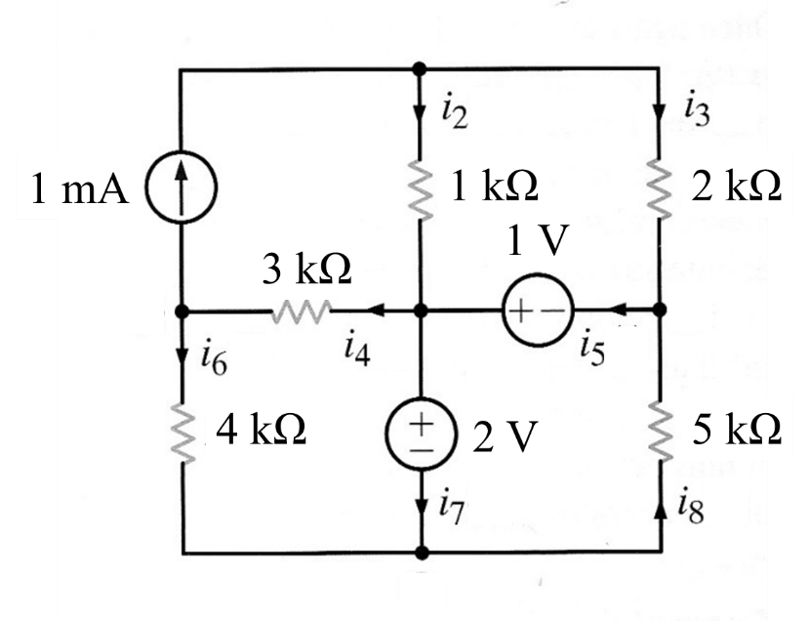
\includegraphics[]{questionbank/networks/circuit_001/v0/schematic.png}
\end{center}

% =========================================================
\begin{partquestion}{unknowns}
{How many unknowns are in the circuit?}
\begin{answer}
There are 7 unknown currents and 6 unknown voltages (don’t forget the voltage across the current source!).
\end{answer}
\end{partquestion}

% =========================================================
\begin{partquestion}{kcl}
{How many KCL equations?}
\begin{answer}
    There are 4 KCL equations (one for all but one node).
\end{answer}
\end{partquestion}

% =========================================================
\begin{partquestion}{kvl}
{How many KVL equations?}
\begin{answer}
There are 4 KVL equations (one for each independent loop).
\end{answer}
\end{partquestion}

% =========================================================
\begin{partquestion}{ohm}
{How many Ohm’s law equations?}
\begin{answer}
There are 5 Ohm’s law equations, one for each resistor.
\end{answer}
\end{partquestion}

% =========================================================
\begin{partquestion}{solve}
{Using variables like $V_{3k}$ to denote the voltage across the 3 kΩ resistor, find all the unknown voltages (in V) and currents (in mA). Leave your answers in a reduced fraction form.}

\begin{answer}
The four KCL equations are (here, current into a node is positive, and current out is negative):
\begin{gather}
-i_2 - i_3 + \qty{1}{\milli\ampere} = 0 \\
i_3 - i_5 + i_8 = 0 \\
i_2 - i_4 + i_5 - i_7 = 0 \\
i_4 - i_6 - \qty{1}{\milli\ampere} = 0
\end{gather}

The four KVL equations are (here the loops were taken in a clockwise fashion):
\begin{gather}
-\qty{1}{\volt} - V_{1k} + V_{2k} = 0 \\
\qty{1}{\volt} - \qty{2}{\volt} - V_{5k} = 0 \\
\qty{2}{\volt} - V_{4k} - V_{3k} = 0 \\
-V_{1\mathrm{mA}} + V_{1k} + V_{3k} = 0
\end{gather}

The five Ohm’s law equations are:
\begin{align}
i_2 &= \frac{V_{1k}}{\qty{1}{\kilo\ohm}} \\
i_3 &= \frac{V_{2k}}{\qty{2}{\kilo\ohm}} \\
i_4 &= \frac{V_{3k}}{\qty{3}{\kilo\ohm}} \\
i_6 &= \frac{V_{4k}}{\qty{4}{\kilo\ohm}} \\
i_8 &= \frac{V_{5k}}{\qty{5}{\kilo\ohm}}
\end{align}

Here is one path to solving the circuit. Starting with (6) it is clear that
$V_{5k} = -\qty{1}{\volt}$.

Next, take (9) and (10) and substitute into (1). After clearing out denominators and rearranging, this gives:
\[
2V_{1k} + V_{2k} = 2
\]

Consider this equation along with (5)—two equations and two unknowns which readily reveal that:
\[
V_{1k} = \frac{1}{3}\,\mathrm{V}, \quad
V_{2k} = \frac{4}{3}\,\mathrm{V}
\]

Next, take (11) and (12) and substitute into (4). After clearing denominators and rearranging, this gives:
\[
4V_{3k} - 3V_{4k} = 12
\]

Consider this equation along with (7)—again two equations and two unknowns which leads to:
\[
V_{3k} = \frac{18}{7}\,\mathrm{V}, \quad
V_{4k} = -\frac{4}{7}\,\mathrm{V}
\]

Using the previous two results plugged into (8) gives:
\[
V_{1\mathrm{mA}} = V_{1k} + V_{3k}
= \frac{1}{3} + \frac{18}{7}
= \frac{61}{21}\,\mathrm{V}
\]

With all voltages determined, we can use Ohm’s law equations to solve for currents:

(9) gives
\[
i_2 = \frac{V_{1k}}{\qty{1}{\kilo\ohm}} = \frac{1}{3}\,\mathrm{mA}
\]

(10) gives
\[
i_3 = \frac{V_{2k}}{\qty{2}{\kilo\ohm}} = \frac{2}{3}\,\mathrm{mA}
\]

(11) gives
\[
i_4 = \frac{V_{3k}}{\qty{3}{\kilo\ohm}} = \frac{6}{7}\,\mathrm{mA}
\]

(12) gives
\[
i_6 = \frac{V_{4k}}{\qty{4}{\kilo\ohm}} = -\frac{1}{7}\,\mathrm{mA}
\]

(13) gives
\[
i_8 = \frac{V_{5k}}{\qty{5}{\kilo\ohm}} = -\frac{1}{5}\,\mathrm{mA}
\]

From (2), we find:
\[
i_5 = i_3 + i_8 = \frac{2}{3} - \frac{1}{5} = \frac{7}{15}\,\mathrm{mA}
\]

From (3), we find:
\[
i_7 = i_2 + i_5 - i_4
= \frac{1}{3} + \frac{7}{15} - \frac{6}{7}
= -\frac{2}{35}\,\mathrm{mA}
\]

In summary, the determined values are:

\begin{table}[htbp]
\centering
\renewcommand{\arraystretch}{1.15}
\begin{tabular}{|c|c|}
\hline
\textbf{Quantity} & \textbf{Value} \\ \hline

$V_{1k}$ & $\tfrac{1}{3}\,\mathrm{V}$ \\ \hline
$V_{2k}$ & $\tfrac{4}{3}\,\mathrm{V}$ \\ \hline
$V_{3k}$ & $\tfrac{18}{7}\,\mathrm{V}$ \\ \hline
$V_{4k}$ & $-\tfrac{4}{7}\,\mathrm{V}$ \\ \hline
$V_{5k}$ & $\qty{-1}{\volt}$ \\ \hline
$V_{1\mathrm{mA}}$ & $\tfrac{61}{21}\,\mathrm{V}$ \\ \hline

$i_2$ & $\tfrac{1}{3}\,\mathrm{mA}$ \\ \hline
$i_3$ & $\tfrac{2}{3}\,\mathrm{mA}$ \\ \hline
$i_4$ & $\tfrac{6}{7}\,\mathrm{mA}$ \\ \hline
$i_5$ & $\tfrac{7}{15}\,\mathrm{mA}$ \\ \hline
$i_6$ & $-\tfrac{1}{7}\,\mathrm{mA}$ \\ \hline
$i_7$ & $-\tfrac{2}{35}\,\mathrm{mA}$ \\ \hline
$i_8$ & $-\tfrac{1}{5}\,\mathrm{mA}$ \\ \hline

\end{tabular}
\end{table}

\end{answer}
\end{partquestion}

\end{mainquestion}